\chapter{Análisis}

\section{Introducción}
El objetivo principal de la ingenieria de requerimientos es crear y mantener un documento sólido de requerimientos del sistema. El proceso general corresponde a cuatro subprocesos de alto nivel de la ingeniería de requerimientos :

<<<<<<< HEAD
\begin{enumerate}
	\item Estudio de viabilidad
	\item \emph{Obtención y análisis}
	\item Especificación
	\item Validación 
\end{enumerate} 
=======
Para abordar cualquier proyecto que se desee desarrollar, debe ser sometido a un infructuoso proceso de análisis, y esto se debe principalmente a que es imposible empezar una construcción sin tener unos planos, que ayuden como guía en el proceso, no solo de hacer una construcción, sino asegurando que sea un desarrollo robusto, y además que asegure un mantenimiento posterior.

Es por esto que en el presente capítulo, se dedicará a describir el análisis de cada requerimiento, mostrando el proceso en cada aspecto tratado en nuestro proyecto.

\newpage
>>>>>>> c216004fa9aef3707abec455c62eef0bebd9aa4c

El foco en esta etapa es la obtención y el análisis, en esta parte del proceso los ingenieros de software interactuan con los clientes y usuarios finales para determinar el dominio de la aplicación , es decir, ¿qué servicios deberá ofrecer?, ¿qué rendimiento se requiere?, ¿para qué hardware? , entre otras cosas. \cite{sommerville2005ingenieria}\\

El término Stakeholder define a todas las personas o grupos que se verán afectados por el sistema, de manera directa o indirecta. A veces comprender y obtener los requerimientos por parte de los stakeholders es complicado por varias razones, por ejemplo, no se conoce lo que se desea del sistema en términos específicos, se habla muy a grandes rasgos pero a la hora de limitar bien y especificar no hay claridad; el lenguaje natural de los clientes y usuarios finales entra en conflicto muchas veces con el lenguaje de los ingenieros (tecnisismos) ; muchos stakeholders, muchos requerimientos diferentes (que tienen corcondancias y conflictos ) y finalmente la dinámica de los requerimientos.\\

<<<<<<< HEAD
Para abordar cualquier proyecto que se desee desarrollar, debe ser sometido a un infructuoso proceso de análisis, y esto se debe principalmente a que es imposible empezar una construcción sin tener unos planos, que ayuden como guía en el proceso, no solo de hacer, sino asegurando que sea un desarrollo y siseño robusto, y además que asegure un mantenimiento a lo largo del tiempo.Es por esto que en el presente capítulo, se dedicará a describir el análisis de cada requerimiento, mostrando el proceso en cada aspecto tratado en nuestro proyecto.



\section{Diagrama de Casos de Uso}
Los casos de uso  y el diagrama de uso de caso UML ayudan a determinar la funcionalidad
y características del software desde la perspectiva del usuario. Un caso de uso describe la manera en la que un usuario interactúa con el sistema, definiendo
los pasos requeridos para lograr una meta específica .Tenga en cuenta que la contribución más importante que hace el caso de uso al desarrollo de software es la descripción textual de cada caso de uso, no el diagrama de uso de caso
global. Es a través de las descripciones que usted puede tener una comprensión clara
de las metas del sistema que desarrolla.\cite{pressman1988ingenieria}

\begin{figure}[h!]
	\centering
	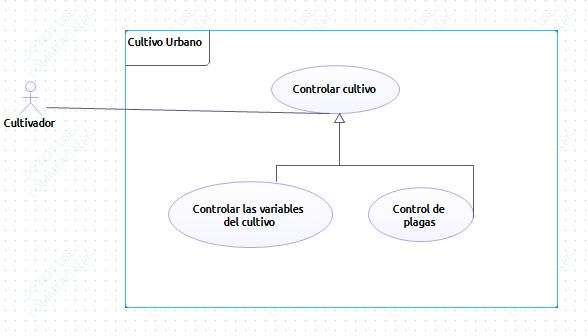
\includegraphics[width=0.7\linewidth]{proyecto/imgs/CasoDeUso}
	\caption{Caso de uso general}
	\label{fig:casodeuso}
\end{figure}

\begin{table}[]
	\centering
	\caption{Requerimiento específico del riego del cultivo.}
=======
\begin{figure}[h!]
	\centering
	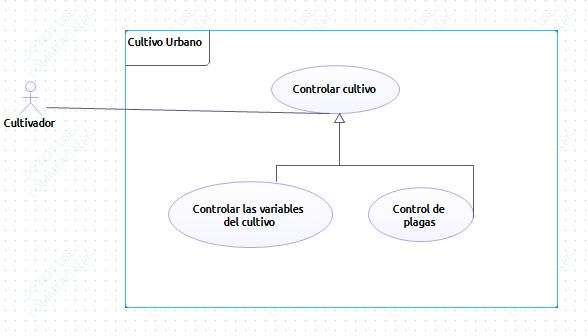
\includegraphics[width=0.7\linewidth]{proyecto/imgs/CasoDeUso}
	\caption{Diagrama de Casos de Uso}
	\label{fig:cronograma}
\end{figure}


\subsection{Requerimientos Específicos}

\begin{table}[h!]
	\centering
	\caption{Requerimiento específico del riego del cultivo.}
	\label{my-label}
	\begin{tabular}{|
			>{\columncolor[HTML]{7BD4EE}}c |c|c|}
		\hline
		{\color[HTML]{000000} \textbf{Nombre}}                   & Riego del cultivo                                                         & ID : 1                                                       \\ \hline
		{\color[HTML]{000000} \textbf{Objetivo}}                 & \multicolumn{2}{c|}{\begin{tabular}[c]{@{}c@{}}Controlar y medir la cantidad\\  de agua suministrada a las plantas\end{tabular}}         \\ \hline
		{\color[HTML]{000000} \textbf{Actores}}                  & \multicolumn{2}{c|}{Cultivador}                                                                                                          \\ \hline
		{\color[HTML]{000000} \textbf{Escenario Primario}}       & \multicolumn{2}{c|}{Se hace el riego de manera exitosa}                                                                                  \\ \hline
		{\color[HTML]{000000} \textbf{Escenario Secundario}}     & \multicolumn{2}{c|}{\begin{tabular}[c]{@{}c@{}}El riego no se lleva a cabo de\\  manera exitosa. (Exceso y Deficit)\end{tabular}}        \\ \hline
		{\color[HTML]{000000} \textbf{Escenarios Excepcionales}} & \multicolumn{2}{c|}{\begin{tabular}[c]{@{}c@{}}- No se dispone de agua .\\ - El sistema de riego no funciona. \\ - Lluvias\end{tabular}} \\ \hline
	\end{tabular}
\end{table}


\begin{table}[h!]
	
	\centering
	\caption{Requerimiento especifico de la iluminación del cultivo}
>>>>>>> c216004fa9aef3707abec455c62eef0bebd9aa4c
	\label{my-label}
	\begin{tabular}{|
			>{\columncolor[HTML]{7BD4EE}}c |c|c|}
		\hline
<<<<<<< HEAD
		{\color[HTML]{000000} \textbf{Nombre}}                   & Riego del cultivo                                                         & ID : 1                                                       \\ \hline
		{\color[HTML]{000000} \textbf{Objetivo}}                 & \multicolumn{2}{c|}{\begin{tabular}[c]{@{}c@{}}Controlar y medir la cantidad\\  de agua suministrada a las plantas\end{tabular}}         \\ \hline
		{\color[HTML]{000000} \textbf{Actores}}                  & \multicolumn{2}{c|}{Cultivador}                                                                                                          \\ \hline
		{\color[HTML]{000000} \textbf{Escenario Primario}}       & \multicolumn{2}{c|}{Se hace el riego de manera exitosa}                                                                                  \\ \hline
		{\color[HTML]{000000} \textbf{Escenario Secundario}}     & \multicolumn{2}{c|}{\begin{tabular}[c]{@{}c@{}}El riego no se lleva a cabo de\\  manera exitosa. (Exceso y Deficit)\end{tabular}}        \\ \hline
		{\color[HTML]{000000} \textbf{Escenarios Excepcionales}} & \multicolumn{2}{c|}{\begin{tabular}[c]{@{}c@{}}- No se dispone de agua .\\ - El sistema de riego no funciona. \\ - Lluvias\end{tabular}} \\ \hline
	\end{tabular}
\end{table}



% Please add the following required packages to your document preamble:
% \usepackage[table,xcdraw]{xcolor}
% If you use beamer only pass "xcolor=table" option, i.e. \documentclass[xcolor=table]{beamer}
\begin{table}[]
	\centering
	\caption{My caption}
	\label{my-label}
	\begin{tabular}{|
			>{\columncolor[HTML]{7BD4EE}}c |c|c|}
		\hline
		{\color[HTML]{000000} \textbf{Nombre}}                   & Iluminación del cultivo                                                                                 & ID : 2                                                                                \\ \hline
		{\color[HTML]{000000} \textbf{Objetivo}}                 & \multicolumn{2}{c|}{\begin{tabular}[c]{@{}c@{}}Controlar la cantidad e intensidad de\\ luminosidad que recibe el cultivo\end{tabular}}                                                          \\ \hline
		{\color[HTML]{000000} \textbf{Actores}}                  & \multicolumn{2}{c|}{Cultivador}                                                                                                                                                                 \\ \hline
		{\color[HTML]{000000} \textbf{Escenario Primario}}       & \multicolumn{2}{c|}{\begin{tabular}[c]{@{}c@{}}El cultivo recibe la cantidad de luz\\  necesaria que garantice su crecimiento \\ óptimo\end{tabular}}                                           \\ \hline
		{\color[HTML]{000000} \textbf{Escenario Secundario}}     & \multicolumn{2}{c|}{\begin{tabular}[c]{@{}c@{}}La luz solar se incrementa a causa \\ de un verano y sequía\end{tabular}}                                                                        \\ \hline
		{\color[HTML]{000000} \textbf{Escenarios Excepcionales}} & \multicolumn{2}{c|}{\begin{tabular}[c]{@{}c@{}}- El sistema que brinda \\ luz y sombra al\\  cultivo deja de funcionar\\ -Obstáculos externos que impidan\\ la llegada de la luz.\end{tabular}} \\ \hline
	\end{tabular}
\end{table}

% Please add the following required packages to your document preamble:
% \usepackage[table,xcdraw]{xcolor}
% If you use beamer only pass "xcolor=table" option, i.e. \documentclass[xcolor=table]{beamer}
\begin{table}[]
=======
		{\color[HTML]{000000} \textbf{Nombre}}                   & Iluminación del cultivo                                                                                 & ID : 2                                                                                \\ \hline
		{\color[HTML]{000000} \textbf{Objetivo}}                 & \multicolumn{2}{c|}{\begin{tabular}[c]{@{}c@{}}Controlar la cantidad e intensidad de\\ luminosidad que recibe el cultivo\end{tabular}}                                                          \\ \hline
		{\color[HTML]{000000} \textbf{Actores}}                  & \multicolumn{2}{c|}{Cultivador}                                                                                                                                                                 \\ \hline
		{\color[HTML]{000000} \textbf{Escenario Primario}}       & \multicolumn{2}{c|}{\begin{tabular}[c]{@{}c@{}}El cultivo recibe la cantidad de luz\\  necesaria que garantice su crecimiento \\ óptimo\end{tabular}}                                           \\ \hline
		{\color[HTML]{000000} \textbf{Escenario Secundario}}     & \multicolumn{2}{c|}{\begin{tabular}[c]{@{}c@{}}La luz solar se incrementa a causa \\ de un verano y sequía\end{tabular}}                                                                        \\ \hline
		{\color[HTML]{000000} \textbf{Escenarios Excepcionales}} & \multicolumn{2}{c|}{\begin{tabular}[c]{@{}c@{}}- El sistema que brinda \\ luz y sombra al\\  cultivo deja de funcionar\\ -Obstáculos externos que impidan\\ la llegada de la luz.\end{tabular}} \\ \hline
	\end{tabular}
\end{table}


\begin{table}[h!]
>>>>>>> c216004fa9aef3707abec455c62eef0bebd9aa4c
	\centering
	\caption{Requerimiento específico del pH del cultivo}
	\label{my-label}
	\begin{tabular}{|
			>{\columncolor[HTML]{7BD4EE}}c |c|c|}
		\hline
		{\color[HTML]{000000} \textbf{Nombre}}                   & Estabilidad del Ph del cultivo                                                                  & ID : 3                                                                \\ \hline
		{\color[HTML]{000000} \textbf{Objetivo}}                 & \multicolumn{2}{c|}{\begin{tabular}[c]{@{}c@{}}Controlar y estabilizar el nivel de  pH  \\ de la tierra usada en el cultivo\end{tabular}}                               \\ \hline
		{\color[HTML]{000000} \textbf{Actores}}                  & \multicolumn{2}{c|}{Cultivador}                                                                                                                                         \\ \hline
		{\color[HTML]{000000} \textbf{Escenario Primario}}       & \multicolumn{2}{c|}{\begin{tabular}[c]{@{}c@{}}El cultivo tiene el pH adecuado \\ para el optimo crecimiento \\ de la planta dependiendo de su tipo.\end{tabular}}      \\ \hline
		{\color[HTML]{000000} \textbf{Escenario Secundario}}     & \multicolumn{2}{c|}{}                                                                                                                                                   \\ \hline
		{\color[HTML]{000000} \textbf{Escenarios Excepcionales}} & \multicolumn{2}{c|}{\begin{tabular}[c]{@{}c@{}}El nivel del pH es bajo debido a : \\ -Nivel de fertilización del cultivo\\ -Lluvias Ácidas\\ -Entre otras\end{tabular}} \\ \hline
	\end{tabular}
\end{table}
<<<<<<< HEAD
\section{Interacciones}
=======
>>>>>>> c216004fa9aef3707abec455c62eef0bebd9aa4c

\newpage

\subsection{Diagrama de Secuencia}
El diagrama de secuencia es uno de los diagramas de representación de comportamiento. Indica la forma en la que los eventos provocan transiciones de un objeto a otro. Luego de identificar los objetos mediante el análisis del caso de uso, se puede representar el flujo que estos tienen uno con otro en un lapso de tiempo.\\

Un diagrama de secuencia se usa para mostrar las comunicaciones dinámicas entre objetos durante la ejecución de una tarea. Este tipo de diagrama muestra el orden temporal en el que los mensajes se envían entre los objetos para lograr dicha tarea. Puede usarse un diagrama de secuencia para mostrar las interacciones en un caso de uso o en un escenario de un sistema de software.
Es importante el desarrollo del diagrama de secuencia porque de esta forma, los eventos que causan transiciones entre objetos del sistema se recopilan en un conjunto de eventos de entrada y de salida (desde un objeto). Esta información es útil en la generación de un diseño eficaz para el sistema que se está elaborando. \cite{bruegge2002ingenieria}

\begin{figure}[h!]
	\centering
	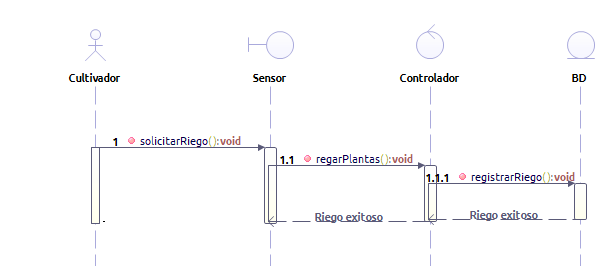
\includegraphics[width=1.2\linewidth]{proyecto/imgs/SecuenciaRiego}
	\caption{}
	\label{fig:secuenciariego}
\end{figure}

\begin{figure}[h!]
	\centering
	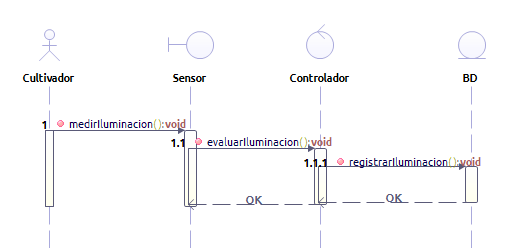
\includegraphics[width=1\linewidth]{proyecto/imgs/SecuenciaIluminacion}
	\caption{}
	\label{fig:secuenciailuminacion}
\end{figure}

\begin{figure}
	\centering
	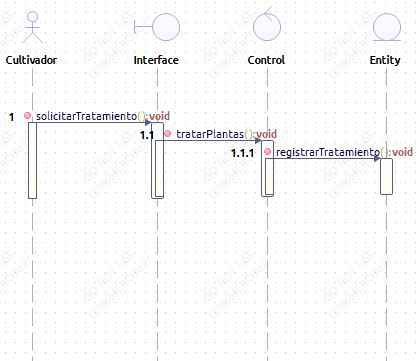
\includegraphics[width=1\linewidth]{proyecto/imgs/SecuenciaTierra}
	\caption{}
	\label{fig:secuenciatierra}
\end{figure}


\begin{figure}[h!]
	\centering
	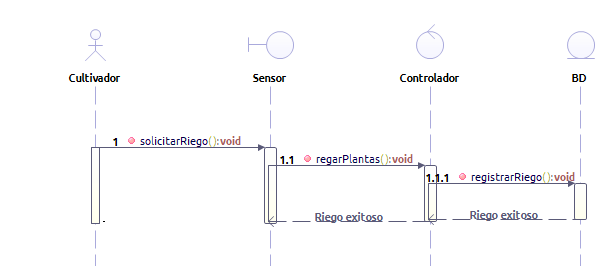
\includegraphics[width=1.0\linewidth]{proyecto/imgs/SecuenciaRiego}
	\caption{Diagrama de Secuencia Riego}
	\label{fig:secuenciariego}
\end{figure}

\begin{figure}[h!]
	\centering
	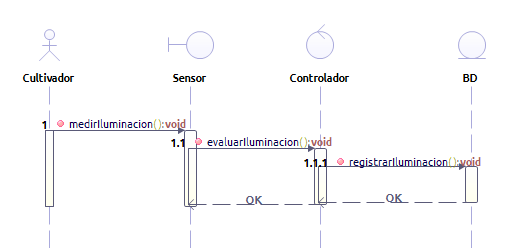
\includegraphics[width=1.0\linewidth]{proyecto/imgs/SecuenciaIluminacion}
	\caption{Diagrama de Secuencia Iluminación}
	\label{fig:secuenciailuminacion}
\end{figure}

\begin{figure}[h!]
	\centering
	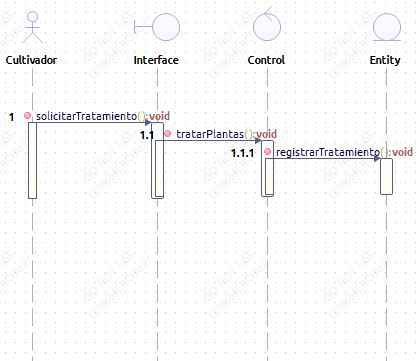
\includegraphics[width=1.0\linewidth]{proyecto/imgs/SecuenciaTierra}
	\caption{Diagrama de Secuencia pH}
	\label{fig:secuenciatierra}
\end{figure}

\newpage

\subsection{Diagrama de Comunicación}

\begin{figure}
	\centering
	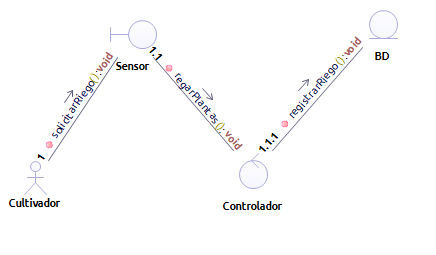
\includegraphics[width=0.8\linewidth]{proyecto/imgs/comunicacionRiego}
	\caption{}
	\label{fig:comunicacionriego}
\end{figure}


\begin{figure}
	\centering
	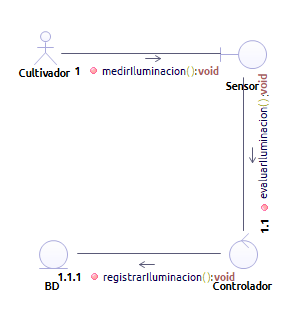
\includegraphics[width=0.6\linewidth]{proyecto/imgs/comunicacionIluminacion}
	\caption{}
	\label{fig:comunicacioniluminacion}
\end{figure}

\begin{figure}
	\centering
	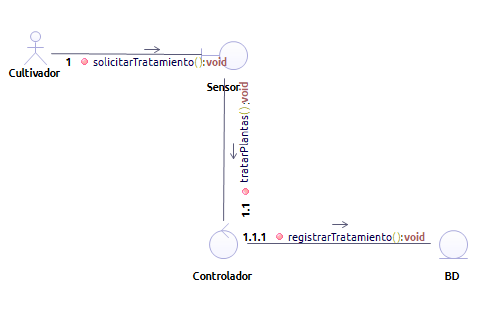
\includegraphics[width=0.8\linewidth]{proyecto/imgs/comunicacionTierra}
	\caption{}
	\label{fig:comunicaciontierra}
\end{figure}
\section{Diagramas de Clases}
El diagrama de clases brinda una visión estática o de estructura de un sistema, sin mostrar la naturaleza dinámica de las comunicaciones entre los objetos de las clases. \cite{bruegge2002ingenieria}
Su importancia recae en la abstracción que brinda al problema, puesto que en él se puede ver las funcionalidades que brinda el sistema (análisis), como también el cómo puede ser construido el sistema (diseño). 
El diagrama muestra las clases del sistema y sus interrelaciones que hay entre los atributos, los cuales son objetos que conocen algo de dicha clase y puede proporcionarlo en todo momento, y las operaciones o comportamientos de la clase, que básicamente es lo que los objetos de la clase pueden hacer.

\subsection{Diagrama de Temporización}

\newpage



\section{Diagramas de Actividades}

\newpage

\section{Diagramas de Workflow}

\newpage

\section{Diagramas de Descripción de la Interacción}

\newpage